\documentclass[runningheads]{llncs}

%\usepackage{times}
%\usepackage{epsfig}
\usepackage{graphicx}
\usepackage{caption}
%\usepackage{subfigure}
\usepackage{subcaption}
\captionsetup{compatibility=false}
\usepackage{amsmath}
\usepackage{amssymb}
\usepackage{ruler}
\usepackage{color}
%\usepackage{pgfplots}
\usepackage[width=122mm,left=12mm,paperwidth=146mm,height=193mm,top=12mm,paperheight=217mm]{geometry}
%\newtheorem{proposition}{Proposition}
%\newtheorem{lemma}{Lemma}
%\newtheorem{proof}{Proof}
\newcommand{\RR}{\mathbb R}
\newcommand{\NNN}{\mathcal N}
\newcommand{\sumi}{\displaystyle{\sum_{i=1}^n}}
\DeclareMathOperator*{\argmin}{argmin}

% Highlighting
\usepackage{soul}
\usepackage{color}
%\usepackage[usenames,dvipsnames]{xcolor}
\newcommand{\hlc}[2][yellow]{{\sethlcolor{#1}\hl{#2}}}
\newcommand{\RAF}[1]{\hlc[yellow]{(RR:) #1}}
\newcommand{\JZ}[1]{\hlc[pink]{(JZ:) #1}}
\newcommand{\PP}[1]{\hlc[green]{PP: #1}}

\usepackage{tikz}
\usepackage{pgfplots}
\pgfplotsset{grid=major,height=2in, width=0.45\columnwidth}

\begin{document}
% \renewcommand\thelinenumber{\color[rgb]{0.2,0.5,0.8}\normalfont\sffamily\scriptsize\arabic{linenumber}\color[rgb]{0,0,0}}
% \renewcommand\makeLineNumber {\hss\thelinenumber\ \hspace{6mm} \rlap{\hskip\textwidth\ \hspace{6.5mm}\thelinenumber}}
% \linenumbers


\pagestyle{headings}
\mainmatter
\def\ECCV16SubNumber{***}  % Insert your submission number here

\title{Kernel Square-Loss Exemplar Machines For Image Retrieval} % Replace with your title

\titlerunning{ECCV-16 submission ID \ECCV16SubNumber}

\authorrunning{ECCV-16 submission ID \ECCV16SubNumber}

\author{Anonymous ECCV submission}
\institute{Paper ID \ECCV16SubNumber}


\maketitle
%\thispagestyle{empty}

%%%%%%%%% ABSTRACT
\begin{abstract}
 In this paper, we propose an improvement to the Exemplar SVM (ESVM) feature encoding pipeline first proposed by Zepeda and P\'erez \cite{ZePe15}. We first show that, by replacing the hinge loss by the square-loss in the ESVM cost function, we obtain similar results on image retrieval in a fraction of the execution time. We call this method Square-Loss Exemplar Machine, or SLEM. Secondly, we introduce a kernelized SLEM variant that, while likewise benefitting from reduced complexity relative to ESVM, further results in a performance avantage in image retrieval. Both SLEM variants exploit the fact that only the exemplar image changes in the training set, and hence most of the SLEM computational complexity can be incurred offline by exploiting the Woodbury matrix identity.  We further propose using a Chlolesky low-rank approximation of the kernel matrix to further reduce SLEM complexity \JZ{We present if for the non-linear case, but should work for the linear case too, no?}. Our experiments establish the performance and computational advantages of our methods using a large array of state-of-the-art base feature representations, and well-known image retrieval dataset.
\end{abstract}

\section{Introduction}

Effective image 
representations are a crucial component of image retrieval systems 
where, given some query image,  images must be retrieved from a large 
database, then ranked according to their degree of similarity with the 
query.
%Robust image representations are a crucial component of a vast number of computer vision applications. 
%Within these, the \emph{image retrieval} application is an important example wherein a query image is provided to the system, which must in turn find all matching images from within a large, unannotated database. 
The matching process is done entirely based on the pixel content of the query and database images, and the search must be robust to large image variations due to camera pose, color differences and scene illumination, amongst others.


The success of several existing systems in this challenging application has been enabled by advances in image representation. 
%An image representation function commonly maps a given input image to a vector in a fixed dimensional space called the image \emph{feature vector}. 
Indeed, once the feature space is given,
the image retrieval process is reduced to finding the feature vectors closest to the query image under, \textit{e.g.}, the Euclidean distance. An adequate image representation must be robust to image variations with preferrably low computation and storage cost.

%A now pervasive example of an image feature representation is that consisting of the activation coefficients extracted from the previous-to-last layer of Convolutional Neural Networks (CNNs) \cite{Krizhevsky2012}. Although CNNs are trained in a fully-supervised manner for the image classification task, they have been shown to transfer well not only to new, unseen classes \cite{Oquaba,Chatfield2014}, but also to alternate tasks such as object detection \cite{Girshick2014} and, importantly, image retrieval \cite{Sharif}.

Many successful feature representations for image retrieval rely on unsupervised models such as $K$-means \cite{Delhumeau2013} or Gaussian mixture models \cite{Perronnin2010}. Very few methods \cite{Arandjelovic15,Bilen2015,Rana} exist that exploit supervised learning of image features directly for the image retrieval task. One of the main reasons for this is the lack of adequately large and varied supervised datasets that are expensive to collect.

The exemplar support vector machine (ESVM), originally proposed by Malisiewicz {\it et al.} \cite{Malisiewicza}, leverages the availability of large, unannotated pools of images within the context of supervised learning. It uses a large generic pool of images as a set of negative examples, while using a single image (the \emph{exemplar}) as a positive example. Given these training set, a linear classifier is learned that can  generalize well, despite the drastically limited size of the set of positive examples.

Zepeda \emph{et al.} \cite{ZePe15} proposed to instead treat the weights of the resulting linear classifier as a new feature vector for the exemplar image. %This new ESVM feature is derived from \emph{base} feature representations ({\it e.g.,} CNN activation features) of the exemplar and the negative pool.
%An extension \cite{ZePe15} of the ESVM formulation discussed above instead treats the resulting linear classifier as an \emph{enhanced} representation of the image feature representing the exemplar image (the \emph{base} feature representation).
An ESVM feature is extracted from each database image, as well as from the query image, by treating each image as an exemplar while keeping a fixed pool of generic negative images. Searching amounts to computing distances between the query and the database ESVM features. Note that ESVM features can be derived from arbitrary \emph{base} features ({\it e.g.} CNN activations) of the exemplar and the images in the generic negative pool. An interesting interpretation of this approach is that the ESVM features represent what is unique about the exemplar relative to the pool of generic negatives, which is the role of a classifier.


One important drawback of the ESVM feature encoding approach is that computing the  classifier requires solving an optimization problem for each positive example. This can be time consuming for large negative pool sizes required for good ESVM feature performance. In this work we propose using the square loss instead of the hinge loss, in effect converting the ESVM problem into a ridge regression that can be solved in closed form. The parameters of the corresponding classifier, which we call the squared loss exemplar machine (SLEM), had been noted to generalize LDA \cite{Koba15} and are shown to form features with comparable performance while drastically reducing the computational cost.


Since computing the SLEM features requires inverting a large matrix related to the training set's scatter matrix, we propose an efficient way to compute this inverse that exploits the fact that only a single (positive) example changes in the training set when computing SLEM features for different images. We show experimentally that our representation can match and even improve upon the performance of ESVM features on two well known datasets using a wide range of base features.

We further introduce a kernel variant of SLEM that enjoys similar computational advantages but improves retrieval performances. \emph{Part about low rank decomposition that I removed.}


The rest of this paper is organized as follows:
%In Section \ref{prior work} we provide an overview of various existing feature representation methods. 
In Section \ref{lsesvm} we first review the original ESVM feature representation method and subsequently introduce the proposed linear SLEM methodd. We then introduce the non-linear SLEM variant in Section \ref{nonlinear SLEM}. We then present the low-rank approximation of our method that enables efficient implementations in the non-linear case in  Section \ref{eff_imp}. We evaluate our proposed method in image retrieval in Section \ref{eval}, and present conclusions in Section \ref{conclusion}.

% Image search
% - Importance.
% - Feature representations. 

% Feature representation - supervised learning
% - Generic framework.
% - Deep CNN features.
% - ImageNet.

% Image retrieval
% - Supervised - Eusipco, NetVLAD.
% - VLAD, Fisher.
% - Cheaper.

% Pool:
% LDA
% SVMs for feature representations - parts learning, Malizsiewics


%\section {Introduction}
% The exemplar SVM (E-SVM) was first introduced by Malisiewicz et al. in \cite{Efros11} as a conceptually simple framework for object detection and image classification where the training set has a small ratio of positive/negative examples. 
% At training time, many SVMs are learned from a large pool of negative against a single positive (so called exemplar). 
% At test time, the scores of the test images for each classifier are fitted by a logistic regression. 
% The final score of an image is then a non-linear combination of scores from multiples exemplar SVMs.

% They have also been used in \cite{Efros12} in image retrieval tasks, using the classifier score to rank matching candidates.
% However this transfer of information from classification to retrieval is severely limited. 
% Indeed, the purpose of a support vector machine is to separate positive and negative samples, i.e., predict discrete labels. 
% The distance between a negative sample and the classification hyperplane has no value as a measure of has \emph{a priori} no value of continuous matching score.

% Zepeda et al. address this problem in \cite{ZePe15} by firstly, performing an E-SVM to each image in a dataset instead of only for the query images and secondly, comparing its classifiers distance to the query's classifier instead of comparing scores. 
% These modifications guarantee we are ranking distances between two points instead of classification scores.
% Therefore \cite{ZePe15} refers to E-SVMs as features encoders: a pipeline that takes an image representation as input and returns an improved image representation. This type of feature enhancing is more akin to methods such as whitening, PCA and LDA.

% This paper introduces the square-loss Exemplar machine (SLEM), which consists of optimizing the same cost function of a regular E-SVM where the hinge loss is replaced by the square loss. 
% The square loss version has the advantage of having a much more efficient optimization. Indeed, the minimization of its cost function is solved by a linear system and can be done for all exemplar simultaneously, whereas the regular E-SVM cost function is generally minimized one exemplar at a time, normally by stochastic gradient descent \cite{bottou10}.
% Also, for the machine learning tasks of binary classification, both regular SVM and least-squares SVM have similar performances \cite{YeXi07}.
% %Also, for the machine learning tasks of binary classification, both regular SVM and least-squares SVM have the same performance if positive and negative samples are separable and the pool of samples is linearly independent \cite{YeXi07}. 
% We also introduce a kernelized version of SLEM, efficiently implemented, that gives better results and superior scalability for large-scale image retrieval problems.

%%% Local Variables:
%%% TeX-master: "main_eccv"
%%% End:


\section{Prior work}
\label{prior work}

\begin{verbatim}
Classic features:
-----------------
VLAD
Fisher Vector
Triangulation embedding
Tolias

Enhancements:
-------------
Spatial Pyramid Pooling (SPP)
Hellinger kernel / root SIFT
Dense sampling
E-SVM

New features:
-------------
CNN features
NetVLAD

Hybrid pooling CNN / aggregator features:
-----------------------------------------
VLAD orderless pooling (exploits SPP)
Conv layers + aggregator: Vedaldi, Kulkarni
SIFT + FCs: Perronin
unsup dense: Deep Fisher vector.


Kernel methods
--------------
\end{verbatim}

% \emph{\color{red} paragraph about image search}

% The image retrieval litterature 

% %where the query image is the positive example and the rank of an search result image is the score of the score of this image in the classifier obtained by the E-SVM. 

% The application of kernel methods for SVM has an extensive bibliography. \emph{\color{red} so extensive that I do not know yet what to put here...}

%%% Local Variables:
%%% TeX-master: "main_eccv"
%%% End:

\section{Squared loss exemplar machine}\label{lsesvm}

In this section, we revisit the exemplar SVM model as presented by \cite{Efros11} and introduce its squared loss version.
\subsection{Exemplar SVMs} \label{esvm}
Given base features in $\RR^d$ at training time, one positive example $x_0$ in $\RR^d$ and a set of negative examples $X = [x_1, x_2,...,x_n]$ in $\RR^{d\times n}$, each column of $X$ representing one example by a vector in $\RR^d$. 
Any feature vector representation can be used.
We are also given a loss function $l:\{-1, 1\}\times \RR\rightarrow\RR^+$. Learning an ESVM from these examples amounts to minimizing the function 
\begin{equation}
J(\omega, \nu) = \theta \ l(1, \omega^Tx_0+\nu) +\dfrac{1}{n}\sumi l(-1, \omega^T x_i+\nu)+\dfrac{\lambda}{2}\|\omega\|^2, \label{eq:first}
\end{equation}
w.r.t. $\omega$ in $\RR^d$ and $\nu$ in $\RR$. In Equation (\ref{eq:first}), $\lambda$ and $\theta$ are respectively a regularization parameter on $\omega$ and a positive scalar adjusting the weight of the positive exemplar.
%\footnote{We could also acknowledge a parameter $\theta$ other than $\frac{1}{n}$ as a regularization to the error of each negative example. But this parameters seems to be less important to cross-validate. Also, setting $\theta=\frac{1}{n}$ simplify Equation (\ref{omega:solution}) and allows the use of Woodbury identity.} 

The  exemplar SVM of $x_0$ with respect to $X$ is the classifier $\omega^\star(x_0,X)$ that minimizes the loss function $J$:
\begin{equation}
\big(\omega^\star(x_0, X), \nu^\star(x_0, X)\big) = \underset{(\omega,\nu)\in\RR^d\times\RR}{\argmin} \ J(\omega, \nu). \label{omega:first}
\end{equation}
To shorten the notation, we refer to these solutions as $\omega^\star$ and $\nu^\star$ when their arguments are implicit.

Applications of ESVM use the hinge loss function, which guarantees that $J$ is a convex function. The solution of Equation (\ref{omega:first}) can be thus found by stochastic gradient descent.

\subsection{Squared loss function}\label{SLEM}
Now, let us study the same learning problem for the squared loss function $l(y,\hat{y}) = \frac{1}{2}(y-\hat{y})^2$. As for the hinge loss, Equation (\ref{eq:first}) is a convex problem. 
However, differently from the hinge loss, it is now a ridge regression problem, whose solution is expressed in a closed form:
\begin{align}
\begin{cases}
\vspace{3 mm}
\omega^\star &= \dfrac{2\theta}{\theta+1}U^{-1}(x_0-\mu), \\
%\vspace{3 mm}
\nu^\star &= \dfrac{\theta-1}{\theta+1}-\dfrac{1}{\theta+1}(\theta x_0+\mu)^T\omega^\star,
\end{cases}
\label{omega:solution}
\end{align}
%\begin{align}
%\nu^\star &= \dfrac{\theta-1}{\theta+1}-\dfrac{1}{\theta+1}(\theta x_0+\mu)^T\omega^\star, \label{eq:nustar}\\
%\omega^\star &= \dfrac{2\theta}{\theta+1}U^{-1}(x_0-\mu) \label{eq:wstar}
%\end{align}
where:
\begin{align}
&\mu = \frac{1}{n}\sum_{i=1}^n x_i,\\
&U = \dfrac{1}{n}XX^T-\mu\mu^T+\dfrac{\theta}{\theta+1}(x_0-\mu)(x_0-\mu)^T+\lambda\mathrm{Id}_d. \label{eq:U}
\end{align}
Equation \ref{omega:solution} shows how to solve (\ref{eq:first}) in a closed form to obtain the SLEM vector $\omega^\star(x_0,X)$ of $x_0$. 
Replacing the hinge loss by the squared loss offers a more compact solution, but not necessarily more efficient.

\subsection{Woodbury identity and matching scores}
Let us define $A = \frac{1}{n}XX^T-\mu\mu^T +\lambda\mathrm{Id}_d$ and assume $A^{-1}$ known. 
%$A$ is the covariance matrix of the negative samples $X$\footnote{added of a small term proportional to the identity matrix to insure $A$ is positive-definite.}. Let us assume its inverse $A^{-1}$ is known. 
Matrix $U$ now reads $U = A + \frac{\theta}{\theta+1}\delta\delta^T$, where $\delta=x_0-\mu$. The Woodbury identity \cite{woodbury} gives us
\begin{equation}
U^{-1} = A^{-1} -\dfrac{\theta}{\theta\delta^TA^{-1}\delta+ \theta+1}A^{-1}\delta^T\delta A^{-1}. \label{invU}
\end{equation}

Using (\ref{invU}) in (\ref{omega:solution}) yields
\begin{equation}
\begin{split}
\omega^\star &= \dfrac{2\theta}{\theta+1}U^{-1}\delta \\
&= A^{-1}\delta - \dfrac{\theta}{\theta\delta^TA^{-1}\delta+ \theta+1} A^{-1}\delta (\delta^TA^{-1}\delta)\\
&= \dfrac{2\theta}{\theta\delta^TA^{-1}\delta+ \theta+1} A^{-1}\delta.\label{Wood:omega}
\end{split}
\end{equation}

The first observation we make from Equation (\ref{Wood:omega}) is that the positive sample weight $\theta$ does not influence the direction of the optimal vector $\omega^\star$, only its norm. This means that if search and ranking are based on the \textit{cosine similarity}, as in \cite{ZePe15}, $\theta$ does not influence the matching score of the SLEM vectors of two different images.
Indeed, if $\omega$ and $\omega'$ are the $d$-dimensional SLEM vectors of $x$ and $x'$, respectively, their cosine similarity reads:
%we can denote $s$ the matching score scalar function defined in $\RR^d\times \RR^d$, which is given by
\begin{equation}
s(\omega, \omega') = \dfrac{\omega^T \omega'}{\|\omega\| \|\omega'\|} = \frac{(x-\mu)^TA^{-2}(x'-\mu)}{\|A^{-1}(x-\mu)\|\|A^{-1}(x'-\mu)\|},\label{match:score}
\end{equation}
which does not depend on the value of $\theta$. This means that the weight of the positive sample can be fixed at any positive value without changing matching scores. This sets the SLEM apart from ESVM that requires this parameter to be cross validated \cite{Efros11,ZePe15}.

%\RAF{I cut the LDA and SLEM section, too long and but particularly useful}
%\subsection{LDA and SLEM}

%Let us now reanalyse the SLEM problem and suppose that we have multiple positive samples. It can be shown that in this case, the corresponding linear classifier of Equation (\ref{eq:first}) for the square-loss is also given by
%(\ref{omega:solution}), where $x_0$ denotes this time the center of mass
%of the positive samples, {\em if} these samples have the {\em same} covariance matrix $\Sigma$ as the negative samples $X$.
 
%This equal-covariance assumption is of course quite restrictive, and probably unrealistic in general. It is interesting to note, however, that this is exactly the assumption made by linear discriminant analysis. As shown in~\cite{Hastie2009} for example, LDA can be seen as a (non-regularized) linear classifier with decision function $\omega^T z+ b'$, where $z$ is a sample in
%$\RR^d$, and
%\begin{equation}
%\left\{\begin{array}{l}
%\displaystyle \omega'=\Sigma^{-1}(x_0-\mu),\\
%\displaystyle b'=-\frac{1}{2}(x_0+\mu)^T \omega',
%\end{array}\right.
%\label{eq:lda}
%\end{equation}
 
%Note that when $\lambda=0$ in SLEM (no regularization),
%\begin{align}
%\Sigma \omega & = U\omega -\frac{1}{2}[(x_0-\mu)^T \omega] (x_0-\mu) =
%\left[1-\frac{1}{2}(x_0-\mu)^T \omega\right](x_0-\mu) \\
%&=\left[1-\frac{1}{2}(x_0-\mu)^T \omega\right]\Sigma \omega'
%\end{align}
%thus $\omega$ and $\omega'$ have the same direction \PP{Not sure to get it. What is $\omega$ here? $\omega^{\star}$? Also it says that $\Sigma \omega$ and $\Sigma \omega'$ are aligned, not $\omega$ and $\omega'$.}.\RAF{This subsection is not particularly important, and can be removed if it is deemed innecessary.} In other words, a
%SLEM is a generalized version of LDA when the
%regularizer parameter $\lambda $ is zero.
%This observation has been equally made by \cite{Koba15}\PP{For square loss e-svm as well?}\RAF{Yes, he briefly studied the E-SVM with square-loss}.

%Many interesting properties of LDA has been rediscovered for classification tasks \cite{GMPD12,HMR12} and, more recently, for image retrieval with non-embedded image encoders \cite{babenko15}.



%%% Local Variables:
%%% TeX-master: "main_eccv"
%%% End:


\section{Kernel methods for SLEM}
\label{nonlinear SLEM}

Let us recall a few basic facts about kernel methods for supervised
classification. We consider a reproducing kernel Hilbert space (RKHS)
$H$ formed by real functions over some set
$X$, and denote by $k$ the corresponding reproducing kernel. Space $H$ is endowed with an inner product $\langle \cdot, \cdot \rangle$ and associated norm $\|\cdot \|$.

We address the following learning problem over $H\times\RR$:
\begin{equation}
\min_{h\in H,\nu\in\RR}
\sum_{i=1}^n l(y_i,h(x_i)+\nu) + \frac{\lambda}{2}\|h\|^2,
\label{eq:kernel}
\end{equation}  
where the pairs $(x_i,y_i)\in X\times \{-1,1\}$, $i=1\dots n$ are training samples, and $l: \{-1,1\}\times \RR\rightarrow\RR^+$ is some arbitrary loss function. 
By definition of a reproducing kernel,
Equation (\ref{eq:kernel}) can be rewritten as
\begin{equation}
\min_{h\in H,\nu\in\RR}
\sum_{i=1}^n l(y_i,\langle \varphi(x_i),h\rangle+\nu) +
\dfrac{\lambda}{2}\|h\|^2,
\label{ker:aff}
\end{equation} 
where $\varphi$ is the {\em feature map} over $X$ associated with the
kernel $k$ (which may not admit a known explicit form). %and $\langle \cdot, \cdot \rangle$ is the inner product of $H$. 
We dub problems with the general form of (\ref{ker:aff}) {\em affine}
supervised learning problems since, given some fixed element $h$ of
$H$ and some scalar $\nu$, $\langle h,h'\rangle+\nu$ is an affine function of $h'$,
whose zero set defines an affine hyperplane of $H$ considered itself
as an affine space.

Let $K$ denote the kernel matrix with entries $k_{ij}=\langle\varphi(x_i),
\varphi(x_j)\rangle$ and rows $k_i^T=[k_{i1}, k_{i2},...,k_{in}]$, $i$ in $\{1,\ldots,n\}$.  We assume from now on that $l$ is convex and continuous. Under this assumption, Equation (\ref{ker:aff}) admits an equivalent formulation
\begin{align}
\min_{\alpha\in\RR^{n},\nu\in\RR} \left(\dfrac{1}{n}\sumi l(y_i, k_i^T\alpha+\nu)  +\dfrac{\lambda}{2}\alpha^TK\alpha\right), \label{ker:first}
\end{align}
and any solution $(\alpha^\star,\nu^\star)$ to (\ref{ker:first})
provides
a solution $(h^\star,\nu^\star)$ to (\ref{ker:aff}) with
$h^\star=\sum_{i=1}^n \alpha_i^\star\varphi(x_i)+\nu^\star$. This result follows from the representer theorem
~\cite{SHS01,Wahba90}.


%where $K$ is a $(n+1)\times (n+1)$  matrix and $k_i$ is its $(i+1)$-th column matrix for $i$ in $\{0, 1, ..., n\}$.\\

Let us assume from now on that $K$ is a semidefinite positive matrix
%\footnote{\textit{i.e.} for any $z$ in $\RR^n$, $z^TKz\ge 0$. This is equivalent to all eigenvalues of $K$ being non-negative.} 
of rank $r$. Its Cholesky decomposition reads $K=BB^T$, with $B$ a rank $r$ upper triangular matrix of size $n\times r$. Using this decomposition, the kernelized problem can be rewritten as 
\begin{equation}
\min_{\beta\in\RR^r,\nu\in\RR} \left( \dfrac{1}{n}\sumi l(y_i, b_i^T\beta+\nu)+\dfrac{\lambda}{2}\|\beta\|^2\right), \label{beta:first}
\end{equation}
where $b_i^T$ denotes the $i$-th row of $B$.

\subsection{Adding a positive exemplar}
\label{subsec:adding}
Let us reconsider the exemplar problem, with one positive example $x_0$ and $n$ negative examples $X$. Here $K$ is the kernel matrix in $\RR^{n\times n}$ of the negative samples $X$. 
Let us also assume its Cholesky factorization $K=BB^T$ is given as well as the pseudoinverse $B^\dagger$ of its factor. We further analyse how to compute $B$ in Subsection~\ref{low-rank}.

We denote $K'$ the augmented kernel matrix obtained by adding the positive samples $x_0$. Such matrix can be written as
\begin{equation}
K' = \begin{bmatrix}
k_{00} & k_0^T\\
k_0 & K
\end{bmatrix},
\end{equation}
where $k_{00}=\langle \varphi(x_0),\varphi(x_0)\rangle$ is a scalar and $k_0= [\langle \varphi(x_0),\varphi(x_i)\rangle]_{1\le i\le n}$ is a vector in $\RR^n$. 
The following lemma shows that the rank $r+1$ Cholesky factorization of $K'$ can be derived from the Cholesky factorization of its sub-matrix $K$.

\begin{lemma} The augmented kernel matrix $K'$ can be factorized as $K'= B'B'^T$ with
%\begin{align}
%K'&= B'B'^T,\quad\text{where}\quad
%B'=\begin{bmatrix}
%u & v^T\\0 & B
%\end{bmatrix}\\
%v&=B^\dagger k_0,\,\, u=\sqrt{k_{00}-||v||^2}.\label{eq:lemma1}
%\end{align}
\begin{equation}
B'=\begin{bmatrix}
u & v^T\\0 & B
\end{bmatrix},~
v = B^\dagger k_0,~ u=\sqrt{k_{00}-||v||^2}.
\label{eq:lemma1}
\end{equation}
\end{lemma}\label{lemma1}
\begin{proof}
For $B'$ defined by (\ref{eq:lemma1}), we have that
\begin{equation}
B'B'^T = 
\begin{bmatrix} u^2+\|v\|^2 & v^TB^T\\ 
Bv& BB^T\end{bmatrix} 
=\begin{bmatrix} k_{00} & v^TB^T\\ 
Bv& K\end{bmatrix} .
\end{equation}
Since $K'$ is positive semidefinite, $k_0$ must lie in the column space $\mathcal{B}$ of $B$.
%\footnote{
Indeed, if we suppose $k_0$ does not belong to $\mathcal{B}$, then it can be decomposed uniquely as $k_0=s+t$, $s\in\mathcal{B}$ and  $t\in\mathcal{B}^\perp$, with $t\ne 0$. In one hand, $K'$ being semidefinite positive implies that $[1, -at^T]K'[1; -at]=k_{00}-2a||t||^2\ge 0$ for all real value $a$. In the other hand, for $a$ large enough, $k_{00}-a||t||^2\le 0$, which is a contradiction.
%} 
Hence $v=B^\dagger k_0$ is an exact solution of $Bv=k_0$. The fact that $k_{00}-\|v\|^2$ is non-negative comes from the fact that the Schur complement $K-k_0 k_0^T / k_{00}$ of $k_{00}$ in $K'$ is itself positive semidefinite.
%\footnote{
Indeed, since the matrix $k_{00}K-k_0k_0^T=B(k_{00}\mathrm{Id}_r-vv^T)B^T$ is positive semidefinite and $B$ has rank $r$, $k_{00}\mathrm{Id}_r-vv^T$ is also positive semidefinite. Thus $v^T(k_{00}\mathrm{Id}_r-vv^T)v = ||v||^2(k_{00}-||v||^2)\ge 0$.
%}
\end{proof}
This lemma allows us to kernelize Equation (\ref{omega:first}) for any positive exemplar $x_0$ and a fixed set of negatives $X$:
%$\beta^\star(x_0,X), \nu^\star(x_0,X) = \underset{\beta\in\RR^{r+1}, \nu\in\RR}{argmin}J'(\beta, \nu)$, for
$\big(\beta^\star(x_0,X),\nu^\star(x_0,X)\big)\in\RR^{r+1}\times\RR$ is the minimizer of $J'(\beta, \nu)$, where
\begin{align}
J'(\beta, \nu)=
 \theta\ l(1, b_0'^T\beta+\nu) +\dfrac{1}{n}\sumi l(-1,b_i'^T\beta+\nu)
+\dfrac{\lambda}{2}\|\beta\|^2,\label{beta:final}
\end{align}
and $b_i'^T$ is the $(i+1)$-th row of $B'$, $i$ in $\{0,1,...,n\}$. In particular, $b_0'=[u; \ v]$ and, for $i>0$, $b_i'=[0; \ b_i]$. Solution $(\beta^\star,\nu^\star)$ can be computed just as before by Equation (\ref{omega:solution}), replacing $x_0$ by $b_0'$, $X$ by the $(r+1)\times n$ matrix $Q$ of columns $b_1', b_2',...,b_n'$ and $\mu$ by $\mu' = \frac{1}{n}\sum_{i=1}^n b_i'$.


\subsection{Matching score}
Once the optimal parameters $(\beta, \nu)$ from (\ref{beta:final}) and the coordinates $u$, $v$ of $b_0'$ from (\ref{eq:lemma1}) have been found\footnote{We drop the ``$\star$'' in this subsection to avoid clutter up the notation.}, they can be used directly for measuring similarity between images. 
Indeed, the corresponding vector $\alpha$ (or, more correctly, \textit{a} corresponding vector of dimension $n+1$) can be computed by $\alpha = P'\beta$, where $P'=B'(B'^TB')^{-1}$  is the pseudoinverse of $B'^T$. This identity can be written as 
\begin{equation}
\begin{bmatrix} \alpha_0 \\ \hat{\alpha} \end{bmatrix} = \begin{bmatrix} \frac{1}{u} & 0^T \\-\frac{1}{u}Pv & P  \end{bmatrix} \begin{bmatrix}\beta_0 \\ \hat{\beta} \end{bmatrix},
\end{equation}
for $P$ pseudoinverse of $B^T$, $\alpha_0$ and $\beta_0$ scalars. The kernalized SLEM of base feature $x_0$ finally reads:
\begin{equation}
h =\alpha_0 \varphi(x_0)+\sum_{i=1}^n \alpha_i \varphi (x_i)+\nu \in H.
\end{equation}
Inspired by the matching score of \cite{ZePe15}, the matching score $s(h,h')$ between $h$ and the encoding $h'=\alpha_0'\varphi(x_0')+\sum_{i=1}^n \alpha_i'\varphi (x_i)+\nu'$ of an other image $x_0'$, is given by (ignoring biases $\nu$ and $\nu'$ which have empirically no influence): 
%\PP{So, biases $\nu$ and $\nu'$ are ignored?}\RAF{Yes, adding it to the classifier does not change the results in a significant way.} 
\begin{equation}
\begin{split}
s(h,h') & = \langle h, h'\rangle \\
		& = \hat{\alpha}^{T} K\hat{\alpha}'+\alpha_0k(X, x_0)^T\hat{\alpha}'+\alpha_0'k(X, x_0')^T\hat{\alpha}+\alpha_0\alpha_0'k(x_0,x_0')\\
		& = \hat{\beta}^T\hat{\beta}'+\frac{\beta_0\beta_0'}{uu'}(k(x_0,x_0')-v^Tv').
\end{split}
\end{equation}



%%% Local Variables:
%%% TeX-master: "main_eccv"
%%% End:



\section{Efficient implementation}\label{eff_imp}
When compared with the problem of (\ref{omega:first}), one drawback of a kernelized approach of (\ref{ker:first}) is that the dimension of our problem grows with the size $n$ of the negative samples.
We can compute the Cholesky factor $B$ of $K$ in $O(nr^2)$ time and $O(nr)$ storage, as will be shown in subsection~\ref{low-rank}. 
For each positive exemplar, solving Equation (\ref{beta:final}) amounts to computing $B'$ from Lemma 1, and solving a linear system in $U$, which is a $(r+1)\times (r+1)$ matrix. The first of these is calculated in time $O(nr)$ and the second, $O(r^3)$.

Two ideas allow us to solve the kernelized problem linearly in $n$: low-rank decomposition of the kernel matrix $K$, to diminish the value of $r$ and the Woodbury identity, so we only have to solve one linear system for all positives. 

\subsection{Low-rank decomposition} \label{low-rank}
In this section we start by revisiting the Cholesky algorithm of the construction of $B$, as presented in ~\cite{BaJo05,FiSc01}. 
We denote, for any list of indexes $M$, $N$ in $\{1,2,...,n\}$, $K(M,N)$ the submatrix of $K$ composed of the rows indexed by $M$ and columns indexed by $N$ and $K(M,:)$ the submatrix of $K$ composed by rows indexed by $M$ and all columns.
Let us assume a sequence of indexes $I_r=\{i_1,i_2,\dots ,i_r\}$ from $\{1,2,\dots, n\}$ is known. 
We also denote, for $t$ in $\{1,2,...,r\}$, $I_t=\{i_1,...,i_t\}$ the subset of the $t$ first indexes of $I_r$ and $J_t=\{1,2,...,n\}/ I_t$ the complement of the $t$ first indexes.
$I_r$ is the set of pivots, chosen greedily such that $i_t$ minimizes the error approximation between $B_tB_t^T$ and $K$, where $B_t=B(I_t,:)$. 

Given $I_t$, we can calculate the $t$-th column, $t=1,2,...,r$, of $B$ iteratively:
\begin{align}
\begin{cases}
\vspace{3 mm}
B(i_t, t) = \left(K(i_t,i_t)-\sum_{m=1}^{t-1} B(i_{m},m)  \right)^{\frac{1}{2}},\\
\vspace{3 mm}
B(I_{t-1},t) = 0,\\
B(J_t, t) = \frac{1}{B(i_t,t)}(K(J_t,i_t)  -\sum_{m=1}^{t-1}B(J_t,m)B(i_t,m)
).\end{cases}\label{icd:algo}
\end{align}
The time complexity of the $t$-th interaction is $O(tn)$, thus making the full algorithm $O(nr^2)$ in time. Since $B$ is $n\times r$, storage complexity is $O(nr)$. In particular, \cite{BaJo05} shows us that, for $t$ in $\{1,2,...,r\}$, the error matrix $K-B_tB_t^T$ is a $(n-t)\times (n-t)$ block matrix which is the Schur complement of $K(I_t,I_t)$ in $K$ and zero elsewhere.

For many kernels such as the Gaussian kernel, $K$ can be a full rank matrix. Its Cholesky decomposition is hence a $O(n^3)$ operation in time, which is a prohibitive cost for large negative sets $X$. We propose stopping the algorithm described in (\ref{icd:algo}) after a given number $r'<r$ of steps, and use $B_{r'}$ as an approximation of $B$. We also need to know only the $r'$ first pivots, which we call $I$ from now on. Conversely, we note $J=J_{r'}$. The construction of $B'$ from $B_{r'}$ can be adapted as presented in the following lemma:
%\begin{proposition}
%There is an unique $n\times n$ matrix $L$ such that
%\begin{itemize}
%\item L is symmetric and positive semidefinite,
%\item L(:,I) = K(:,I),
%\item the column space of $L$ is equal to the column space of $L(:,I)$.
%\end{itemize}
%L is such that 
%\begin{equation}
%L([I \ J],[I\ J]) = \begin{bmatrix}
%K(I,I) && K(J,I)^T\\ K(J,I) && K(J,I)K(I,I)^{-1}K(J,I)^T
%\end{bmatrix}.
%\end{equation}
%\end{proposition}
%From \textbf{Proposition 1}, $L$ is an unique approximation of $K$ for a given pair $I$ and $J$. The algorithm from (\ref{icd:algo}) construct $B$ such that $L=BB^T$.
\begin{lemma}
The augmented kernel matrix $K'$ can be factorized as $K'\approx B'B'^T$ where
\begin{equation}
\begin{split}
& B'=\begin{bmatrix} u & v^T\\w & B_{r'} \end{bmatrix},~ v=B_I^{-1} k_0(I),~ u=\sqrt{k_{00}-\|v\|^2},\\
& w(I) = 0,~w(J)=\dfrac{1}{u}(k_0(J)-B_Jv),
\end{split}
\end{equation}
in time $O(nr')$ and storage $O(n)$. Also, the approximation error of $K'$ and $B'B'^T$ is the same of $K$ and $B_{r'}B_{r'}^T$. Here, $B_I$ and $B_J$ denote $B(I,I)$ and $B(J,I)$, respectively.
\end{lemma}
The proof of this lemma is similar to the previous lemma's proof, only adding the $\RR^n$ vector $w$ whose entries are calculated by Equation (\ref{icd:algo}).
%\begin{proof}
%As before, we have that
%\begin{equation}
%B'B'^T = \begin{bmatrix} u+|\!|v|\!|^2 & v^TB_{r'}^T+uw^T\\ 
%B_{r'}v+uw& BB^T+ww^T\end{bmatrix}.
%\end{equation}
%If $E = K'-B'B'^T$,
%Algorithm (\ref{icd:algo}) is such that the rank of $B_{r'}$ is $r'$, for all $r'<r$.
%\end{proof}
\subsection{Woodbury identity}
Let us call $A=\frac{1}{n}QQ^T-\mu'\mu'^T+\lambda\textbf{Id}_{r+1}$, where $Q$ and $\mu'$ are defined at the end of \S \ref{subsec:adding}. We assume its inverse $A^{-1}$ known. From the kernalized version of (\ref{omega:solution}), we know that $U=A+\frac{\theta}{\theta+1}\delta\delta^T$, with $\delta=b_0'-\mu'$. The Woodbury identity gives us 
\begin{equation}
U^{-1}=A^{-1} -\dfrac{\theta}{\theta\delta^TA^{-1}\delta+ \theta+1}A^{-1}\delta^T\delta A^{-1}.\label{wood1}
\end{equation}
Replacing (\ref{wood1}) in the original equation yields the solution
\begin{equation}
\beta^\star = \dfrac{2\theta}{\theta+1}U^{-1}\delta = \dfrac{2\theta}{\theta\delta^TA^{-1}\delta+ \theta+1}A^{-1}\delta,\label{beta:fromwood}
\end{equation}
which depends only $A^{-1}$, $\theta$, $\mu'$ and $b_0'$. 
We can thus solve only one linear system with matrix $A$ for \textit{all} positives, instead of one in $U$ for \textit{each} positive.

If we decompose $K$ at rank $r$, $A$ is constant for all positives, since $Q = [0, B]$ and $\mu'=[0; \mu]$.\footnote{Here, $\mu$ is the center of mass of the rows of $B$, not the columns of $X$ as initially presented in section \ref{lsesvm}.} 
But for a low-rank decomposition, we have instead $Q=[w, B_{r'}]$ and $\mu' = [\bar{w}; \mu]$. If so, $A$ is written as 
\begin{equation}
A = \begin{bmatrix}
a_{00} & a_0^T\\
a_0^T & G
\end{bmatrix},
\end{equation}
where $a_{00}=\dfrac{1}{n}w^Tw-\bar{w}^2+\lambda$, $a_0 = \dfrac{1}{n}B_{r'}^Tw-\bar{w}\mu$ and $G=\dfrac{1}{n}B_{r'}^TB_{r'}-\mu\mu^T+\lambda\text{Id}_r$.

Matrix $G$ depends only on $B$ and can be calculated in time $O(nr'^2)$ and storage $O(r'^2)$. 
Its inverse $G^{-1}$ is computed at cost $O(r'^3)$.
The Woodbury identity, again, allows the computation of $A^{-1}$ from $G^{-1}$ at cost $O(r^2)$:
\begin{equation}
A^{-1} = \begin{bmatrix}\gamma & -\gamma a_0^TG^{-1}\\ -\gamma G^{-1}a_0 & G^{-1}+\gamma G^{-1}a_0a_0^TG^{-1}\end{bmatrix},\label{wood2}
\end{equation}
where $\gamma = \left(a_{00}-a_0^TG^{-1}a_0\right)^{-1}$. Finally, replacing (\ref{wood2}) in (\ref{beta:fromwood}), we can obtain $\beta^\star$ by solving the linear problem $A\beta^\star = \delta$. 
Both $A$ and $\delta$ are dependent on $u$, $v$ and $w$, which are computed for each exemplar as described by Lemma 2.

%%% Local Variables:
%%% TeX-master: "main_eccv"
%%% End:

\section{Experimental Evaluation}
\label{eval}

%% Low-rank, mAP vs. r', n=50e3
%% Temps, 
%% Spatial Pyramid.

\subsection{Datasets and evaluation protocol} \label{eval:protocol}
\subsubsection{Holidays and Oxford5K.} We use two standard image retrieval datasets for our experiments. The first one is the INRIA \emph{Holidays} dataset \cite{holidays}. This dataset consists of 1491 images divided into 500 groups of matching images. %If the dataset of an experiment is not mentioned in what follows this means, by default, that it is performed on \emph{Holidays}.
The second one is  the \emph{Oxford5k} dataset \cite{oxford}, which consists of 5062 images divided into 55 groups of matching images. 

In both datasets, each group contains one query image, the other images in the group being the only correct answers to the query. We use the mAP computation procedures provided along with the dataset to evaluate performance.

\subsubsection{Flickr $1e6$.} Besides these two datasets, we also use $1e6$ random distractor images downloaded from \emph{Flickr} to carry out large scale experiments, following standard protocol \cite{holidays,Delhumeau2013,ZePe15}.

%For each query image, we calculate its similarity to all other images in the database and rank them, in decreasing order.
%The average precision of a group is derived from the ranking of the images of the group for the similarity with the corresponding query image.
%The final mean average precision (mAP) for a dataset is the mean of the average precision over all its groups.
\subsubsection{Negative pool.} As a pool of negative images to build E-SVM and SLEM representations, we use the Flickr100k collection \cite{oxford}, composed of $10^5$ random Flickr images disjoint from those in Flickr $1e6$.. For a full rank decomposition, we use only a subset of it, containing between 6000 and 15000 images.
As stated in section \ref{low-rank} and further discussed in section \ref{time-scale}, a full rank decomposition does not scale well for bigger number of negative samples. For low rank decomposition, we use all 100000 images.

%REMOVED
%At evaluation time, for a dataset that consists of $p$ images and $q$ query images, we calculate its $p\times q$ \emph{similarity matrix} $S$, where each of its $q$ columns is the matching scores of the query image with all the $p$ images.


\subsection{Which kernel to choose?}
We tested four differnt kernels. The first three --linear, Gaussian, polynomial -- are defined below:
\begin{align}
    &k_{linear}(x,y) = x^Ty, \label{k:lin}\\
    &k_{Gauss}(x,y) = \exp(-\gamma\|x-y \|^2), \label{k:rbf}\\
    &k_{poly}(x,y) = x^Ty+\lambda(x^Ty)^2. \label{k:poly}
    %&k_{SPM}(x,y) = \dfrac{1}{2^L}\mathcal{I}(H^0_x, H^0_y) +\sum_{l=1}^L\dfrac{1}{2^{L-l+1}}\mathcal{I}(H^{l,\gamma}_x, H^{l,\gamma}_y). \label{k:spm}
\end{align}
%\JZ{We give results with spp, we should add it. Makes it clear that we use a wide range of kernels.}
%\JZ{The text below could be removed. But some brief text for SPM is a good idea, as it is less standard. I think SPP and SPM are not the same thing... We should use SPM... SPP is a finite dimensional feature map.}
% \textbf{Linear SLEM} The linear kernel of Equation (\ref{k:lin}) is the first default choice and equivalent to the non-kernelized version of SLEM.
% In the remaining of this paper, we reference to linear SLEM when we use the non-kernelized SLEM.
% \textbf{Gaussian SLEM} The radial basis function kernel of Equation (\ref{k:rbf}) is a
% well known reproducing kernel, used for classification with support vector machines.
% \textbf{Polynomial SLEM} The polynomial kernel of Equation (\ref{k:poly}) is a reproducing kernel often used in natural language processing.
%\textbf{SPM SLEM} The spatial pyramid matching kernel of $L+1$ levels in Equation \ref{k:spm} take as input a set of local descriptors and its location in pyramidal bins \cite{spk}. 
Note that Gaussian and polynomial kernels require a scalar parameter ($\gamma$ and $\lambda$, respectively), that we set using cross-validation \JZ{What is the cross-valid dataset?}.

Besides the three kernels above described, we likewise carry out experiments using the Spatial Pyramid Matchin (SPM) kernel.
%The SPM kernel of $L+1$ levels in Equation \eqref{k:spm} takes as input a set of local descriptors and computes a similarity score that takes into account their geometrical layout \cite{spk}.\JZ{Need to define $H_x^{l,\gamma}$ ...}
%its location in pyramidal bins \cite{spk}. 


\subsection{Base visual features}
We test our feature encoder for three different base features $x\in\mathbb{R}^d$ the hand-crafted VLAD image representation \cite{Delhumeau2013} and two learned features derived from the activation coefficients of deep Convolutional Neural Networks \cite{Krizhevsky2012,babenko15}.

We use the same VLAD variant of \cite{Delhumeau2013} used in \cite{ZePe15} that relies on densely-extracted rootSIFT \cite{3things} local descriptors, per-cluster, PCA-based rotations, and root normalization. Like \cite{ZePe15}, we use $64$ clusters, for a final feature size of $8192$.

The first CNN-based feature we use consists of the activation coefficients of the previous-to-last layer of the architecture of \cite{Krizhevsky2012}, based on a publicly available pre-trained model \cite{jia2014caffe}. This is the same feature considered in \cite{ZePe15} and originally considered as an image retrieval feature in \cite{Sharif}. We refer to it as FC-CNN. \JZ{Please verify...}

The second CNN-based feature, the SPoC feature of \cite{babenko15}, is tailored specifically for the image retrieval application. It consists of a spatially-weighted sum-pooling of the activations of the last convolutional layer of a 19-layer CNN \cite{Simonyan2014}.

%REMOVED
% We revisit the VLAD feature presented in \cite{VLAD} as an example of a hand-crafted representation. First we extract a set $\mathcal{F}$ of local descriptors of the image $I$. We use the 128 dimension RootSIFT \cite{3things} descriptors, extracted densely.
% Then, we hard-assign each descriptor $f$ in $\mathcal{F}$ to the closest among $K$ pre-trained codewords $c_k$, $k\in\{1\cdots K\}$,
% %one of $K$ set $\mathcal{C}_k$ of descriptors associated to codewords $\{c_k\}_{1\leq k\leq K}$, 
% and map $f$ to a $\RR^{128K}$ vector
% \begin{equation}
% \phi^{VL}_1(f) = \left[0 \cdots 0\quad \Phi_k^T\frac{(f-c_k)}{\|f-c_k\|} \quad 0 \cdots 0\right],
% \end{equation}
% where $\Phi_k$ is a $128\times 128$ PCA matrix learned on training features mapped to $k$-the codeword.
% %associated to descriptors in $\mathcal{C}_k$. 
% The final VLAD representation is the power-normalization and $l_2$ normalization of the sum-pooling of $\phi^{VL}_1$:
% \begin{equation}
% \phi^{VL}_2(I) \propto \mathrm{power}\big(\sum_{f\in \mathcal{F}}\phi^{VL}_1(f)\big),~\|\phi^{VL}_2(I)\|=1,
% \end{equation}
% with scalar power normalization $\mathrm{power}(v)=\mathrm{sign}(v)|v|^{0.5}$ applied component-wise.
% In experiments, we use $K=64$ codewords learned on images from Flickr. Our VLAD representation has $d=8192$ dimensions.


%REMOVED
% Convolutional features obtained from very deep convolutional neural networks (CNNs) have been shown to work as good local descriptors for matching \cite{SimonZisser15}. The SPoC representation \cite{babenko15} is a weighted sum-pooling of the activations of the last convolutional layer of a 19-layer CNN. For a given input image $I$, the activations in this layer are organized over a $W\times H$ spatial grid and over $d$ channels. Each position $(w,h)\in \{1 \cdots W\}\times \{1\cdots H\}$ can thus be equipped with a descriptor $f_{h,w}(I)\in\RR^D$.
% %Indeed, if our last convolutional layer has $D$ neurons, and each neuron a $W\times H$ map of activations of this neurons to the image $I$, 
% %each pair $(w,h)$ with $w$ in $\{1,2,..., W\}$ and $h$ in $\{1,2,...,H\}$ can be associated to a descriptor $f_{(h,w)}$ in $\RR^D$ of the responses of each neuron at coordinate $(w,h)$ of the maps. 
% We then sum-pool these descriptors, weighted accordingly to their distance to the center of the image:
% \begin{equation}
%     \phi^{SPoC}(I) = \sum_{w=1}^W\sum_{h=1}^H \alpha_{w,h}f_{w,h}(I),
% \end{equation}
% where
% \begin{equation}
%     \alpha_{w,h} = \exp \left(-\dfrac{(w-W/2)^2+(h-H/2)^2}{2\sigma^2}\right).
% \end{equation}
% In our experiments, we follow the implementation details of \cite{babenko15}: We resize all images to $586\times 586$ pixels before feeding them to the network. The last convolutional layer has $d=512$ channels with activation maps of size $(W,H)=(37,37)$. We also set $\sigma=\frac{H}{3}$.

% Finally, we also test a more convencional CNN feature, less deep and using two fully connected layers after the convolutional layers.
% Our final representation is a $4096$ non-negative feature. We based out implementation on CAFFE \cite{jia2014caffe}.


% \subsection{Implementation details}
% We cross validate $\gamma$ and $\lambda$ for Poly and Gaussian SLEM.

%\subsection{Full rank results}
\subsection{Comparison to other enhancement methods using various base features} \JZ{Renamed from ``Full rank results'', not too convinced myself... but if we don't have low-rank results...}
In Table \ref{fullrank:results}, we test our method using the three recent base features discussed above (VLAD \cite{Delhumeau2013}, SPoC \cite{babenko15}, and FC-CNN \cite{Sharif}) and two datasets (6 combinations in total). We further compare against two feature enhancement strategies: {\it ( i)} the ESVM method of \cite{ZePe15}, as well as {\it ( ii)} the PCA+whitening strategy shown in \cite{babenko15} to drastically improve the retrieval results for SPoC. In our experiments, using PCA dimensionality reduction worsens the results, and hence we use the full PCA projection matrix for the PCA+whitening strategy.
%Hence we compare the improvements of PCA plus whitening, without compression, with our method.

Note that our method succeeds in improving the performance of the base feature for all three features tested and on both Holidays and Oxford 5K datasets. It further outperformns both ESVM and PCA+whiteninng feature enhancement strategies in 5 out of 6 cases, by as many as 2.8 mAP points (for SPoC CNN on Oxford 5K). Although nonlinear SLEM enjoys the highest performance, linear SLEM nonetheless outperforms both feature enhancement methods in 4 out of 6 cases illustrated in the table.

%Linear SLEM performs similarly to ESVM despite being much more time efficient (see discussion in section \ref{time-scale}).
%Gaussian SLEM and Polynomial SLEM outperform all methods, for all datasets and all image representations.
%The results are presented in Table \ref{fullrank:results}.

\begin{table*}[t]
\begin{center}
\caption{Mean average precision results for INRIA Holidays and Oxford buildings datasets, expressed as percentages. In this table, we present our results for VLAD-64 \cite{Delhumeau2013}, sum-pooling of convolutional features (SPoC) \cite{babenko15} and fully connected (fc) CNN \cite{jia2014caffe}}
\begin{tabular}{|c|c|c|c|c|c|c|c|}
\hline
Dataset & \multicolumn{3}{|c|}{\textbf{Holidays}} & \multicolumn{3}{|c|}{\textbf{Oxford 5k}}\\
\hline
Method, features & VLAD-64  & SPoC CNN & FC CNN & VLAD-64 & SPoC CNN & FC CNN\\
\hline\hline
Base feature            & 72.7         & 73.1         & 68.2         & 46.3           & 54.4         & 40.6\\
%Whitening           & -    & -    & -    & -    & -\\
PCA+whitening       & 69.4         & 77.5         & 69.2         & 50.9           & 63.7         & 45 \\
E-SVM               & \textbf{77.5} & 79.9         & 71.8         & 57.5           & 62.1         & 44.6\\
Linear SLEM         & 78           & 78.3         & 72.1         & \textbf{59.3}   & 64.1         & 45.5\\
Gaussian SLEM       & 78.1         & 81.4         & \textbf{72.9} & 59             & \textbf{64.9} & 46.1\\
Poly SLEM           & 78.1         & \textbf{82}   & \textbf{72.9} & \textbf{59.3}  & 64.8         & 46\\
\hline
\end{tabular}
\end{center}
\label{fullrank:results}
\end{table*}

\begin{figure}[!h]
\centering
\begin{tikzpicture}
	\begin{semilogxaxis}[
		xlabel=Number of noisy images,
		ylabel=mAP,
		legend = south west]
%%Poly SLEM
    \addplot[PolySLEM] coordinates{
        (   0, 0.5929)
        (1000, 0.5918)
        (3000, 0.5901)
        (6000, 0.5881)
       (10000, 0.5864)
       (30000, 0.5759)
       (60000, 0.5663)
      (100000, 0.5598)
      (300000, 0.5405)
      (600000, 0.5310)
    };
    \addlegendentry{PolySLEM}
	\addplot[ESVM] coordinates{
        (   0, 0.5750)
        (1000, 0.5738)
        (3000, 0.5728)
        (6000, 0.5715)
       (10000, 0.5700)
       (30000, 0.5620)
       (60000, 0.5533)
      (100000, 0.5477)
      (300000, 0.5276)
      (600000, 0.5121)
    };	
    \addlegendentry{RESVM-2}
    %\addplot[VLAD] coordinates{
    %    (   0, 0.463)
    %    (1000, 0.4611)
    %    (3000, 0.4585)
    %    (6000, 0.4558)
    %   (10000, 0.4534)
    %   (30000, 0.4443)
    %   (60000, 0.4372)
    %  (100000, 0.4322)
    %  (300000, 0.4170)
    %  (600000, 0.4050)
    %};
    %\addlegendentry{VLAD}
    \addplot[LinSLEM] coordinates{
        (   0, 0.5933)
        (1000, 0.5922)
        (3000, 0.5904)
        (6000, 0.5883)
       (10000, 0.5860)
       (30000, 0.5751)
       (60000, 0.5643)
      (100000, 0.5588)
      (300000, 0.5385)
      (600000, 0.5260)
    };
    \addlegendentry{LinSLEM}
	\end{semilogxaxis}
\end{tikzpicture}
\caption{mAP for Oxford 5k varying the number of distractors, using SPoC features and different methods of SLEM (see legend).}
\label{vlad:oxford}
\end{figure}



\subsection{Time Scalability} \label{time-scale}
In Figure \ref{fullrank:results} we evaluate the \textit{(left)} mAP performance and \textit{(right)} time efficiency of (non-)linear SLEM as a function of the negative pool size $n$, comparing it to ESVM. To compute mAP for ESVM, we use $T=10^5$ iterations for all values of $n$ to favour performance. Timings for ESVM are those reported in \cite{ZePe15}, but assuming $T=n 10/6$ (the factor of $10/6$ is used in \cite{ZePe15}).

For all features, we report only timings related to ESVM or SLEM feature extraction. For the case of ESVM or linear SLEM, this includes only the computation of the vector of weights $\omega^\star$. For nonlinear SLEM, this includes the computation of all components of Equation \eqref{eq:nl_sim} that involve the query vector $x_0$ (i.e., $\hat \beta, \beta_0, k(x_0, x_0^\prime), u$ and $v$). \JZ{This does depend on the size of the database... We should indicate what database size we are assuming...}

Note that linear SLEM enjoys a considerable computational advantage of close to two orders of magnitude over ESVM, while under-performing by less than two mAP points. Non-linear SLEM, on the other hand uniformly outperforms ESVM in terms of mAP, but incurs a computational penalty for higher negative pool sizes. The increased complexity for Gaussian and polynomial kernels is expected: storing and solving a $n\times n$ system does not scale for large number of negative samples $n$.

%In this section we compare the time efficiency of our method to that of E-SVM,  as discuss which method to use accordingly with the number of positive and negative samples.

%REMOVED this bc now it does change with n...
%In Figure \ref{fullrank:results}, we see that Linear SLEM efficiency does not change with $n$.
%Indeed, if $d$ is the dimension of the base representation, $A$ is a $d\times d$ matrix for Linear SLEM, whereas for a full rank kernel, $A$ is a $n\times n$.

%The reason for the increased complexity for Gaussian and polynomial kernels follows since storing and solving a $n\times n$ system does not scale for large number of negative samples.
%But retrieval results in Figure \ref{fullrank:results} suggest we can benefit from larger sets of negative samples. %Linear SLEM and ESVM scales well, but do not perform so well.

\vspace{3 mm}

\begin{figure}
  \begin{tikzpicture}
    \begin{groupplot}
      [group style={%
        columns=2,
        rows=1,
        group name=plots,
        xlabels at=edge bottom,
        %y descriptions at=all,
        horizontal sep=5em,        
      },
      % ybar,
      % ymin=0,
      % ymax=27e3,
      enlarge x limits={abs=.5},
      width=0.5\textwidth,
      height=0.4\textwidth,
      % scaled y ticks=base 10:-3,
      % xticklabels from table={\first}{Criterion},
      % x tick label style={rotate=90,anchor=east},
      % xtick=data,
      ]

      \nextgroupplot[xlabel=Num. of negatives,
      ylabel=mAP]
      ]
      %% Poly SLEM
      \addplot[PolySLEM] coordinates {
        (500,  0.78852)
        (1500, 0.80397)
        (2500, 0.80648)
        (3500, 0.80905)
        (4500, 0.81192)
        (5500, 0.81502)
        (6500, 0.81659)
        (7500, 0.81712)
        (8500, 0.81599)
        (9500, 0.81432)
        (10500,0.81625)
        (11500,0.81796)
        (12500,0.81726)
        (13500,0.81993)
        (14500,0.82057)
      };
      %% Gaussian SLEM
      \addplot[GaussSLEM] coordinates {
        (500,  0.77757)
        (1500, 0.79756)
        (2500, 0.80338)
        (3500, 0.79909)
        (4500, 0.79950)
        (5500, 0.80257)
        (6500, 0.8016)
        (7500, 0.80362)
        (8500, 0.80377)
        (9500, 0.80501)
        (10500,0.80534)
        (11500,0.80909)
        (12500,0.80955)
        (13500,0.80813)
        (14500,0.81214)
      };
      %% ESVM
      \addplot[ESVM] coordinates {
        (500,  0.7684)
        (1500, 0.78434)
        (2500, 0.78836)
        (3500, 0.78927)
        (4500, 0.79292)
        (5500, 0.79523)
        (6500, 0.79491)
        (7500, 0.79557)
        (8500, 0.79915)
        (9500, 0.79819)
        (10500,0.79888)
        (11500,0.7985)
        (12500,0.79822)
        (13500,0.79930)
        (14500,0.79905)
      };
      %% Linear SLEM
      \addplot[LinSLEM] coordinates {
        (500,  0.77638)
        (1500, 0.7748)
        (2500, 0.77919)
        (3500, 0.77914)
        (4500, 0.7748)
        (5500, 0.77578)
        (6500, 0.77902)
        (7500, 0.78338)
        (8500, 0.78043)
        (9500, 0.78026)
        (10500,0.77803)
        (11500,0.77767)
        (12500,0.77818)
        (13500,0.78148)
        (14500,0.78254)
      };

      \nextgroupplot[
      ymode=log,
      xlabel=Num. of negatives,
      ylabel=Time per image (s),
      legend to name=grouplegend,
      legend style={legend columns=-1},
      % legend style={at={(0.465,-0.45)},
      % anchor=north,legend columns=-1},
      ]%
      %% Poly SLEM
      \addplot[PolySLEM] coordinates {
        (500,  0.0001)
        (1500, 0.0007)
        (2500, 0.0023)
        (3500, 0.0046)
        (4500, 0.0088)
        (5500, 0.0146)
        (6500, 0.0213)
        (7500, 0.0289)
        (8500, 0.0395)
        (9500, 0.0542)
        (10500,0.0703)
        (11500,0.0903)
        (12500,0.1103)
        (13500,0.1434)
        (14500,0.1745)
      };
      \addlegendentry{Poly SLEM}
      %% Gaussian SLEM
      \addplot[GaussSLEM] coordinates {
        (500,  0.0003)
        (1500, 0.0008)
        (2500, 0.0021)
        (3500, 0.0044)
        (4500, 0.0072)
        (5500, 0.0119)
        (6500, 0.0172)
        (7500, 0.026)
        (8500, 0.0344)
        (9500, 0.0465)
        (10500,0.0617)
        (11500,0.0814)
        (12500,0.1248)
        (13500,0.1301)
        (14500,0.161)
      };
      \addlegendentry{Gaussian SLEM}
      %% ESVM
      \addplot[ESVM] coordinates {
        (500,  0.014)
        (1500, 0.015)
        (2500, 0.016)
        (3500, 0.017)
        (4500, 0.018)
        (5500, 0.019)
        (6500, 0.02)
        (7500, 0.021)
        (8500, 0.022)
        (9500, 0.023)
        (10500,0.024)
        (11500,0.025)
        (12500,0.026)
        (13500,0.027)
        (14500,0.028)
      };
      \addlegendentry{ESVM}
      %% Linear SLEM
      \addplot[LinSLEM] coordinates {
        (500,  0.0000565)
        (1500, 0.0000575)
        (2500, 0.0000467)
        (3500, 0.0000679)
        (4500, 0.0000683)
        (5500, 0.0000612)
        (6500, 0.0000608)
        (7500, 0.0000708)
        (8500, 0.0000743)
        (9500, 0.0000996)
        (10500, 0.0000993)
        (11500,0.0001073)
        (12500,0.0001027)
        (13500,0.000075)
        (14500,0.0001141)
      };
      \addlegendentry{Linear SLEM}
      


    \end{groupplot}

    \node at (plots c1r1.north east) [anchor=south, xshift=2.5em] {\ref{grouplegend}};
    %\draw (plots c2r1.north west) circle (3pt) node {North west};

  \end{tikzpicture}
  \caption{Results for INRIA Holidays, using SPoC features and different methods of SLEM (see legend).}
  \label{fullrank:results}
\end{figure}


% \begin{figure}
%   \begin{tikzpicture}
%     \begin{groupplot}
%       [group style={%
%         columns=3,
%         group name=plots,
%         xlabels at=edge bottom,
%         y descriptions at=edge left,
%       },
%       ybar,
%       ymin=0,
%       ymax=27e3,
%       enlarge x limits={abs=.5},
%       width=0.35\textwidth,
%       height=0.6\textwidth,
%       scaled y ticks=base 10:-3,
%       xticklabels from table={\first}{Criterion},
%       x tick label style={rotate=90,anchor=east},
%       xtick=data,
%       ]

%       \nextgroupplot[xlabel=item1,legend to name=grouplegend,ylabel=y-label]
%       \pgfplotstableforeachcolumn\first\as\col{%
%         \ifnum\pgfplotstablecol=0
%         \else
%         \edef\tmp{%
%           \noexpand\addplot table [x expr=\noexpand\coordindex,y=\col] {\noexpand\first};
%           \noexpand\addlegendentry {\col}%
%         }%
%         \tmp
%         \fi
%       }

%       \nextgroupplot[xlabel=item2]
%       \pgfplotstableforeachcolumn\second\as\col{%
%         \ifnum\pgfplotstablecol=0 
%         \else
%         \edef\tmp{%
%           \noexpand\addplot table [x expr=\noexpand\coordindex,y=\col] {\noexpand\second};
%         }%
%         \tmp
%         \fi
%       }

%       \nextgroupplot[xlabel=item3]
%       \pgfplotstableforeachcolumn\third\as\col{%
%         \ifnum\pgfplotstablecol=0 
%         \else
%         \edef\tmp{%
%           \noexpand\addplot table [x expr=\noexpand\coordindex,y=\col] {\noexpand\third};
%         }%
%         \tmp
%         \fi
%       }
%     \end{groupplot}

%     \node at (plots c2r1.north) [anchor=south, yshift=.6cm] {\ref{grouplegend}};
%   \end{tikzpicture}
% \end{figure}


% \def\sideboxwidth{0.48\textwidth}
% \def\centerboxwidth{0.02\textwidth}
% \begin{figure}[!h]
%   \begin{minipage}{\sideboxwidth}
%     \begin{center}
%       \begin{tikzpicture}
% 	\begin{axis}[
%           xlabel=Num. of negatives,
%           ylabel=mAP]
%           %% Poly SLEM
%           \addplot[PolySLEM] coordinates {
%             (500,  0.78852)
%             (1500, 0.80397)
%             (2500, 0.80648)
%             (3500, 0.80905)
%             (4500, 0.81192)
%             (5500, 0.81502)
%             (6500, 0.81659)
%             (7500, 0.81712)
%             (8500, 0.81599)
%             (9500, 0.81432)
%             (10500,0.81625)
%             (11500,0.81796)
%             (12500,0.81726)
%             (13500,0.81993)
%             (14500,0.82057)
%           };
%           %% Gaussian SLEM
%           \addplot[GaussSLEM] coordinates {
%             (500,  0.77757)
%             (1500, 0.79756)
%             (2500, 0.80338)
%             (3500, 0.79909)
%             (4500, 0.79950)
%             (5500, 0.80257)
%             (6500, 0.8016)
%             (7500, 0.80362)
%             (8500, 0.80377)
%             (9500, 0.80501)
%             (10500,0.80534)
%             (11500,0.80909)
%             (12500,0.80955)
%             (13500,0.80813)
%             (14500,0.81214)
%           };
%           %% ESVM
%           \addplot[ESVM] coordinates {
%             (500,  0.7684)
%             (1500, 0.78434)
%             (2500, 0.78836)
%             (3500, 0.78927)
%             (4500, 0.79292)
%             (5500, 0.79523)
%             (6500, 0.79491)
%             (7500, 0.79557)
%             (8500, 0.79915)
%             (9500, 0.79819)
%             (10500,0.79888)
%             (11500,0.7985)
%             (12500,0.79822)
%             (13500,0.79930)
%             (14500,0.79905)
%           };
%           %% Linear SLEM
%           \addplot[LinSLEM] coordinates {
%             (500,  0.77638)
%             (1500, 0.7748)
%             (2500, 0.77919)
%             (3500, 0.77914)
%             (4500, 0.7748)
%             (5500, 0.77578)
%             (6500, 0.77902)
%             (7500, 0.78338)
%             (8500, 0.78043)
%             (9500, 0.78026)
%             (10500,0.77803)
%             (11500,0.77767)
%             (12500,0.77818)
%             (13500,0.78148)
%             (14500,0.78254)
%           };
% 	\end{axis}
%       \end{tikzpicture}
%     \end{center}
%   \end{minipage}%
%   \begin{minipage}{\centerboxwidth}~\end{minipage}%
%   \begin{minipage}{\sideboxwidth}
%     \begin{center}
%       \begin{tikzpicture}
% 	\begin{semilogyaxis}[
%           xlabel=Num. of negatives,
%           ylabel=Time per image (s),
%           legend style={at={(0.465,-0.45)},
%             anchor=north,legend columns=-1},
%           ]%legend pos=outer south]
%           %% Poly SLEM
%           \addplot[PolySLEM] coordinates {
%             (500,  0.0001)
%             (1500, 0.0007)
%             (2500, 0.0023)
%             (3500, 0.0046)
%             (4500, 0.0088)
%             (5500, 0.0146)
%             (6500, 0.0213)
%             (7500, 0.0289)
%             (8500, 0.0395)
%             (9500, 0.0542)
%             (10500,0.0703)
%             (11500,0.0903)
%             (12500,0.1103)
%             (13500,0.1434)
%             (14500,0.1745)
%           };
%           \addlegendentry{Poly SLEM}
%           %% Gaussian SLEM
%           \addplot[GaussSLEM] coordinates {
%             (500,  0.0003)
%             (1500, 0.0008)
%             (2500, 0.0021)
%             (3500, 0.0044)
%             (4500, 0.0072)
%             (5500, 0.0119)
%             (6500, 0.0172)
%             (7500, 0.026)
%             (8500, 0.0344)
%             (9500, 0.0465)
%             (10500,0.0617)
%             (11500,0.0814)
%             (12500,0.1248)
%             (13500,0.1301)
%             (14500,0.161)
%           };
%           \addlegendentry{Gaussian SLEM}
%           %% ESVM
%           \addplot[ESVM] coordinates {
%             (500,  0.014)
%             (1500, 0.015)
%             (2500, 0.016)
%             (3500, 0.017)
%             (4500, 0.018)
%             (5500, 0.019)
%             (6500, 0.02)
%             (7500, 0.021)
%             (8500, 0.022)
%             (9500, 0.023)
%             (10500,0.024)
%             (11500,0.025)
%             (12500,0.026)
%             (13500,0.027)
%             (14500,0.028)
%           };
%           \addlegendentry{ESVM}
%           %% Linear SLEM
%           \addplot[LinSLEM] coordinates {
%             (500,  0.0000565)
%             (1500, 0.0000575)
%             (2500, 0.0000467)
%             (3500, 0.0000679)
%             (4500, 0.0000683)
%             (5500, 0.0000612)
%             (6500, 0.0000608)
%             (7500, 0.0000708)
%             (8500, 0.0000743)
%             (9500, 0.0000996)
%             (10500, 0.0000993)
%             (11500,0.0001073)
%             (12500,0.0001027)
%             (13500,0.000075)
%             (14500,0.0001141)
%           };
%           \addlegendentry{Linear SLEM}
% 	\end{semilogyaxis}
%       \end{tikzpicture}
%       \caption{Results for INRIA Holidays, using SPoC features and different methods of SLEM (see legend).}
%       \label{fullrank:results}
%     \end{center}
%   \end{minipage}
% \end{figure}

%% Local Variables:
%% TeX-master: "main_eccv"
%% End:


%\subsection{Low-rank decomposition evaluation}


%\begin{figure}[!h]
%\centering
%\begin{subfigure}[b]{0.48\textwidth}
%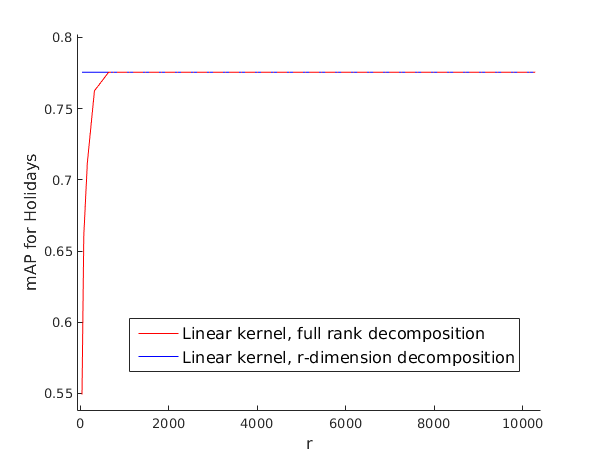
\includegraphics[width=\textwidth]{linear_decomposition_nolog.png}
%\end{subfigure}
%\begin{subfigure}[b]{0.48\textwidth}
%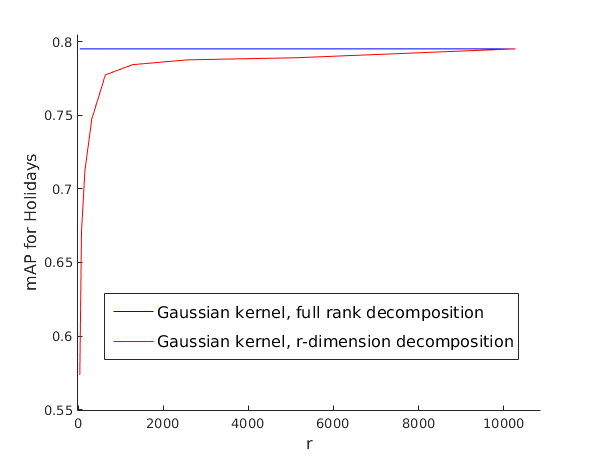
\includegraphics[width=\textwidth]{rbf_decomposition_nolog.png}
%\end{subfigure}
%\caption{Comparison between full rank and low rank. In blue, mAP results for full rank SLEM. %In red, mAP results for low rank decomposition of SLEM, varying the rank $r'$.
%At the left, linear SLEM results;at the right, Gaussian SLEM results. In this experiment, $n=10281$.}
%\label{no.ker.vs.linear2}
%\end{figure}

\subsection{Spatial pyramid matching kernel}

\begin{table}[!h]
    \centering
    \caption{Results for spatial pyramids kernel when compared with a Bag of Visual Words from the local descriptors \JZ{BoW to change to SPM} }
    \begin{tabular}{|c|c|c|c|c|}
    \hline
    Dataset & \multicolumn{2}{|c|}{\textbf{Holidays}} & \multicolumn{2}{|c|}{\textbf{Oxford 5k}}\\
    \hline
        Method, feaures & RootSIFT & CNN & RootSIFT
        &CNN \\
    \hline
    \hline
    Baseline (BoW) & 37.4 & 49.8 & 31.1 & 32.4 \\
        SP SLEM    & 66.9 & 70.2 & 42.4 & 45 \\
    \hline
    \end{tabular}
    \label{tab:spk}
\end{table}
All previous kernel functions take as input image representations in a fixed sized vectorial space. In this section, we propose using the spatial pyramid kernel \cite{GrauDa05}, that takes as input a set of local descriptors and its coordinates in the image.

We revisit the spatial pyramid scheme presented in \cite{spk} using the generalized intersection function of histograms.

Let $X$, $Y$ be the sets of local descriptors of a pair of images.
These local descriptors can be associated to one of $M$ codewords $\{c_1,c_2,...,c_M\}$, so that $X=\bigcup_{1\leq m \leq M}X_m$ and $Y=\bigcup_{1\leq m \leq M}Y_m$, so that $X_m$, $Y_m$ are the set of descriptors associated to $c_m$.
For level $l$ in $\{0,1,..., L\}$, we divide the images in grids $2^l\times 2^l$ and we call $H^{(l,m)}_X$, $H^{(l,m)}_Y$ the $4^l$-dimensional histograms of the occurrences of the of the visual word $c_m$ in each bin of the grid.
The kernel $K_{sp}(X,Y)$ is given by sum over all codewords of the intersection histogram of $H^{(l,m)}_X$ and $H^{(l,m)}_Y$, $l=0,...,L$,  weighted proportionally to the number of bins in each level.

We test this kernel for RootSIFT extracted in multiscales, as used in \cite{spk}, and learn the codewords with K-means. Inspired by the results of \cite{SPPCNN}, we also test it for activations of the last convolutional layer of the network of \cite{SimonZisser15}. Each neuron of the last layer correspont to a codeword. The results are presented in Table \ref{tab:spk}.

%The spatial pyramid kernel is given by
%\begin{align}
%    K_{sp}(X,Y) &= \sum_{m=1}^M \kappa^L(X_m, Y_m), \ where \\
%    \kappa^L(X_m,Y_m) &= 2^{-L}I^{l}(X_m,Y_m) +\sum_{l=1}^L 2^{-L+l-1}I^{l}(X_m,Y_m) \label{kappa}\\
%    I^{l}(X_m,Y_m) = \sum_{i=1}^{4^l}\min()
%\end{align}



%% Local Variables:
%% TeX-master: "main_eccv"
%% End:

\section{Conclusion}
\label{conclusion}
In this paper, we address the problem of large scale image retrieval with global image representation. 
We presented a simples idea, the kernelized squared loss exemplar machine, and yet an elegant implementation. 
As a result, we obtain significant improvement over the image representations we tested, outperform similar encoders and near state of the art performances.
As future work, we must test our method on state of the art representations and see how it impacts their results.
The use of other kernel functions is also encouraged. The polynomial outperforms the Gaussian kernel, even though the Hilbert space obtained from the Gaussian kernel has infinite dimensions \emph{\color{red} fact check}. 
The spatial pyramid kernel can be used to improve representations based on local descriptors


\bibliographystyle{ieee} 
\bibliography{sup,jz}
\end{document}


	
%%% Local Variables:
%%% TeX-master: "main_eccv"
%%% End:
